\documentclass[master=mai,masteroption=ecs]{kulemt}
\setup{title={Fixed Size Least Squares Support Vector Machines: A Scala based programming framework for Large Scale Classification},
  author={Mandar Chandorkar},
  promotor={Prof.\,dr.\,ir.\ Bart De Moor \and Prof.\,dr.\,ir.\ Johan A.K Suykens},
  assessor={Ir.\,Kn. Owsmuch\and K. Nowsrest},
  assistant={Oliver Lauwers \and Dr. Raghvendra Mall}}
% The following \setup may be removed entirely if no filing card is wanted
\setup{filingcard,
  translatedtitle=,
  udc=621.3,
  shortabstract={We propose \textit{FS-Scala}, a flexible and modular \textit{Scala} based implementation of the Fixed Size Least Squares Support Vector Machine (FS-LSSVM) for large data sets. The framework consists of a set of modules for (gradient and gradient free) optimization, model representation, kernel functions and evaluation of FS-LSSVM models. A kernel based \textit{Fixed-Size Least Squares Support Vector Machine} (FS-LSSVM) model is implemented in the proposed framework, while heavily leveraging the parallel computing capabilities of \textit{Apache Spark}. Global optimization routines like \emph{Coupled Simulated Annealing} (CSA) and \emph{Grid Search} are implemented and used to tune the hyper-parameters of the FS-LSSVM model. Finally, we carry out experiments on benchmark data sets like \emph{Magic Gamma} and \emph{Adult} and evaluate the performance of various kernel based FS-LSSVM models.}}
% Uncomment the next line for generating the cover page
%\setup{coverpageonly}
% Uncomment the next \setup to generate only the first pages (e.g., if you
% are a Word user.
%\setup{frontpagesonly}

% Choose the main text font (e.g., Latin Modern)
\setup{font=lm}

% If you want to include other LaTeX packages, do it here. 

% Finally the hyperref package is used for pdf files.
% This can be commented out for printed versions.
\usepackage[pdfusetitle,colorlinks,plainpages=false]{hyperref}
\usepackage{blindtext, tikz, csvsimple, adjustbox}
\usepackage{amsmath}
\usepackage{amsfonts}
\usepackage{amssymb}
\interdisplaylinepenalty=2500
\usepackage{tikzscale, adjustbox}

\usepackage[school]{pgf-umlcd}
\usepackage[ruled,vlined,linesnumbered,inoutnumbered]{algorithm2e}
\usepackage{verbatim} 
\usepackage{booktabs} % For \toprule, \midrule and \bottomrule

\usepackage{siunitx} % Formats the units and values
\usepackage{pgfplotstable} % Generates table from .csv
\usepackage{datatool}

\usepackage{textgreek}

\usepackage{times}
%\usepackage{geometry}

\usetikzlibrary{mindmap, backgrounds,positioning,shapes,shadows,arrows}
\sisetup{
  round-mode          = places, % Rounds numbers
  round-precision     = 2, % to 2 places
}

%%%%%%%
% The lipsum package is used to generate random text.
% You never need this in a real master thesis text!
\IfFileExists{lipsum.sty}%
 {\usepackage{lipsum}\setlipsumdefault{11-13}}%
 {\newcommand{\lipsum}[1][11-13]{\par And some text: lipsum ##1.\par}}
%%%%%%%

%\includeonly{chap-n}
\begin{document}

\begin{preface}
  I would like to thank everybody who kept me busy the last year,
  especially my promoter and my assistants. I would also like to thank the
  jury for reading the text. My sincere gratitude also goes to my wife and
  the rest of my family.
\end{preface}

\tableofcontents*

\begin{abstract}
We propose \textit{FS-Scala}, a flexible and modular \textit{Scala} based implementation of the Fixed Size Least Squares Support Vector Machine (FS-LSSVM) for large data sets. The framework consists of a set of modules for (gradient and gradient free) optimization, model representation, kernel functions and evaluation of FS-LSSVM models. A kernel based \textit{Fixed-Size Least Squares Support Vector Machine} (FS-LSSVM) model is implemented in the proposed framework, while heavily leveraging the parallel computing capabilities of \textit{Apache Spark}. Global optimization routines like \emph{Coupled Simulated Annealing} (CSA) and \emph{Grid Search} are implemented and used to tune the hyper-parameters of the FS-LSSVM model. Finally, we carry out experiments on benchmark data sets like \emph{Magic Gamma} and \emph{Adult} and evaluate the performance of various kernel based FS-LSSVM models.
\end{abstract}

% A list of figures and tables is optional
%\listoffigures
%\listoftables
% If you only have a few figures and tables you can use the following instead
\listoffiguresandtables
% The list of symbols is also optional.
% This list must be created manually, e.g., as follows:
\chapter{List of Abbreviations and Symbols}
\section*{Abbreviations}
\begin{flushleft}
  \renewcommand{\arraystretch}{1.1}
  \begin{tabularx}{\textwidth}{@{}p{12mm}X@{}}
    SVM   & Support Vector Machine \\
    FS-LSSVM   & Fixed Size Least Squares Support Vector Machine \\
    CG   & Conjugate Gradient \\
    CSA  & Coupled Simulated Annealing \\
    AFE  & Automatic Feature Extraction \\
    API  & Application Programming Interface \\ 
    KKT  & Karush Kuhn Tucker \\
    RHKS & Reproducing Kernel Hilbert Space\\
    SVC & Support Vector Classification\\
    SVR & Support Vector Regression\\
    SMO & Sequential Minimal Optimization\\
    QP & Quadratic Programming\\
    ROC & Receiver Operating Characteristic\\
    OOP & Object Oriented Programming\\
    FP & Functional Programming\\
    JVM & Java Virtual Machine\\
  \end{tabularx}
\end{flushleft}
\section*{Symbols}
\begin{flushleft}
  \renewcommand{\arraystretch}{1.1}
  \begin{tabularx}{\textwidth}{@{}p{12mm}X@{}}
    42    & ``The Answer to the Ultimate Question of Life, the Universe,
            and Everything'' according to \cite{h2g2} \\
    $c$   & Speed of light \\
    $E$   & Energy \\
    $m$   & Mass \\
    $\pi$ & The number pi \\
  \end{tabularx}
\end{flushleft}

% Now comes the main text
\mainmatter

\chapter{Introduction}
\label{cha:intro}
The $21^{st}$ century stands out in how mankind learned the value of storing and making predictions/decisions from large volumes of data. A significant aspect of large scale data analysis is distributed computation frameworks like \textit{High Performance Computing}, \textit{Message Passing Interface} etc. Recently large scale commodity hardware clusters have replaced the two former frameworks as the most popular model for parallel data analysis. With this crucial change in hardware came a change in computational models as well. It is at this juncture that distributed \textit{Map Reduce} became the de-facto computational philosophy for large scale data analysis and  words such as \textit{Hadoop} \cite{Hadoop:2005, chang2008bigtable, Borthakur2011} and \textit{Apache Spark} \cite{Zaharia2010, Spark:2010} have become synonymous with large scale data analysis and machine learning.

Along with innovation in hardware design and distributed computing models, there came a need for good programming libraries and frameworks to work with various Machine Learning models on large data sets. It was demonstrated in \cite{10.1109/MIS.2009.36} that a gigantic language corpus encapsulates almost all aspects of human language and speech. So far the prevalent `motto' in the Internet industry has been ``large data, simple models". Often, this is misunderstood as the Machine Learning translation of \textit{Occam's Razor}. The bias-variance trade-off \cite{Valentini2004} (appendix \ref{app:biasvar}) is a far better mechanism to ensure that a model does not become overly complex, and this, rather than restricting the user to simple models, is the real Occam's razor in training a model. 

Therefore, in order to extract maximum value from large scale data, it is important to have the flexibility to train and compare different model families before arriving at the one that fits the requirement of the user. Therefore one must be able to train general nonlinear models and tweak them by changing the various components which they employ to learn (i.e., a model may be linear or kernel based, it can be optimized by various methods like \textit{Stochastic Gradient Descent}, \textit{Conjugate Gradient}, etc.). This is not possible in a rigid, monolithic programming framework. Modularity, extensibility and ease of usage are of paramount importance while designing Machine Learning software for large scale data applications.

Scala \cite{scala-overview-tech-report}, a multi-paradigm Java Virtual Machine (JVM) based programming language has gained popularity for its expressiveness and performance. It's power and easy interpolability with Java has contributed to its adoption in software architectures that heavily rely on Java and its ecosystem. The current state of the art in distributed Machine Learning in Scala is the \textit{MLLib} module in \textit{Apache Spark} \cite{Meng}. It has implementations of Linear SVM and Logistic Regression for solving binary classification problems. But a crucial component missing in \textit{MLLib} and all distributed Machine Learning libraries is the ability to learn classification models with nonlinear decision boundaries. FS-Scala aims to solve the problem of scalable non-linear classification models by implementing the \textit{Fixed-Size Least Squares Support Vector Machine} (FS-LSSVM) algorithm \cite{DeBrabanter2010,Suykens2002} with model tuning capabilities.

In recent literature we find sparse reductions to FS-LSSVM methods \cite{Mall2015,Mall2013}. The authors in \cite{Mall2015,Mall2013} explored the sparsity vs error trade-off \footnote{Sparsity vs error trade off refers to how the model error increases when the number of prototype vectors is reduced via the $L_0$ regularization on model parameters.} for FS-LSSVM models. Even though they run experiments on large scale data sets like \emph{Forest Cover}, the scalability of these methods are restricted to available memory on a single machine. Moreover, they don't exploit the possibility of parallelism available in several components of the FS-LSSVM model. 

Another work \cite{Mall2014} converts the Big Data into a Big Network and then uses a network based subset selection technique (\textit{Fast and Unique Representative Subset selection} (FURS) \cite{Mall2013FURS}) to obtain a representative subset of the original data. It then builds a FS-LSSVM model using this subset. However, in this thesis we showcase that we can distribute the subset selection computation which maximizes the \textit{Quadratic R\`enyi Entropy} for Big data sets and use the generated subset as the set of prototype vectors (PV) essential for building the FS-LSSVM model.

The rest of this thesis is organized as follows.

\begin{itemize}
\item Chapter \ref{cha:1} briefly discusses the classical Support Vector Machine (SVM) as well as the LSSVM formulations. In the case of the LSSVM, the dual formulation is discussed motivating the introduction of the FS-LSSVM which solves the LSSVM in the primal for large data sets.

\item Chapter \ref{cha:2} compares and contrasts various programming languages and paradigms, justifying the choice of Scala in the implementation of the FS-LSSVM. The rest of the chapter focuses on the salient features of the current SVM and LSSVM software implementations and motivates the issues tackled by FS-Scala. Chapter \ref{cha:2} concludes with the contributions of \emph{FS-Scala} in LSSVM software design and implementation.

\item Chapter \ref{cha:3} introduces distributed \emph{MapReduce} and details the computational phases of the FS-LSSVM which are performed in a distributed manner in \emph{FS-Scala}.

\item Chapter \ref{cha:n} discusses experiments conducted using \emph{FS-Scala} on the \emph{Magic Gamma}, \emph{Adult} and \emph{Forest Cover Type} data and tabulates the performance of various kernel based as well as linear FS-LSSVM models on the selected data sets.

\item The thesis concludes \ref{cha:conclusion} with a discussion of the results of experiments of chapter \ref{cha:n} and further research directions that can be pursued with respect to the development of \emph{FS-Scala}.
\end{itemize}

%%% Local Variables: 
%%% mode: latex
%%% TeX-master: "thesis"
%%% End: 

\chapter{Least Squares Support Vector Machines}
\label{cha:1}
%%%%%%%%%%%%%%%%%%%%%%%%%%%%%%%%%%%%%%%%%%%
\section{Least Squares Support Vector Machines} \label{LSSVM}
%%%%%%%%%%%%%%%%%%%%%%%%%%%%%%%%%%%%%%
\subsection{Formulation}
%%%%%%%%%%%%%%%%%%%%%%%%%%%%%%%%%%%%%%%%%%%5
Least Squares Support Vector Machines (LSSVM) \cite{Suykens2002} \cite{Suykens1999} modifies the SVM formulation to include the \textit{squared error} loss function and equality constraints with respect to the error variables $e_i$, as shown in \eqref{eqlssvm}. 
\begin{equation}\label{eqlssvm}
\begin{aligned}
& \underset{w,b,e}{\text{min}}
& & \mathcal{J}(w,e) = \frac{1}{2}w^{\intercal}w + \frac{\gamma}{2}\sum\limits_{i=1}^N e_{i}^2 \\
& \text{s.t.}
& & y_{i}[ w^{\intercal}\phi(x_{i})+b ] = 1 - e_{i}, i=1,\ldots ,N.
\end{aligned}
\end{equation}
%%%%%%%%%%%%%%%%%%%%%%%%%%%%%
Introducing the Lagrangian and applying the KKT conditions gives us the solution of the problem in the dual \eqref{eqkkt}. This solution implies a loss of sparsity as compared to the classical SVM since each point becomes a support vector. However, we gain linearity of the solution (i.e. we do not have to solve the \textit{Quadratic Programming} problem as in the classical SVM). Solving the problem in the dual is not advantageous for large scale analysis as the size of the solution matrix is equal to the size of the original data.  
%%%%%%%%%%%%%%%%%%%%%%%%%%%%%%%%%
\begin{equation}
\label{eqkkt}
\left[\begin{array}{c|c}
   0  & y^\intercal   \\ \hline
   y & \Omega + \gamma^{-1} \mathit{I} 
\end{array}\right] 
\left[\begin{array}{c}
   b    \\ \hline
   \alpha  
\end{array}\right] = \left[\begin{array}{c}
   0    \\ \hline
   1_v  
\end{array}\right],
\end{equation}
%%%%%%%%%%%%%%%%%%%%%%%%%%%%%%%%%%%%%%%%%%%%%%%%%%%5
where $\Omega_{kl} = y_{k}y_{l}K(x_{k}, x_{l})$, $\alpha = \left[\alpha_1 ; ... ; \alpha_N \right]$ and $K(x_k,x_l) = \phi(x_k)^\intercal\phi(x_l)$.
%%%%%%%%%%%%%%%%%%%%%%%%%%%%%%%%%%%%%%%%%%%%%%%%%%%%
\subsection{FS-LSSVM} \label{sec:fs}
In order to make the training of kernel based SVM models for large scale data applications feasible, one needs to make approximations to the computation of the kernel matrices. The Fixed-Size LSSVM (FS-LSSVM) as proposed by De Brabanter, Suykens et. al \cite{DeBrabanter2010,Suykens2002} consists of solving the LSSVM problem in the primal as follows.
%%%%%%%%%%%%%%%%%%%%%%%%%%%%%%
\begin{equation}
\label{eqfs}
\min_{w,b} \ \frac{1}{2}w^{\intercal} w + \frac{\gamma}{2}\sum^{n}_{i=1} \left(y_{i} - w^{\intercal} \hat{\phi}(x_i) - b\right)^{2}.
\end{equation}

The solution to equation \ref{eqfs} is given by:
\begin{align}
\label{eqfssol}
& \left( \begin{matrix}
\hat{w}\\ 
\hat{b}
\end{matrix}\right ) = 
\left ( \hat{\Phi}^{\intercal}_e \hat{\Phi}_e + \frac{\mathit{I}_{m+1}}{\gamma} \right )^{-1} \hat{\Phi}^{\intercal}_e y,
\\ \nonumber \\
\text{where} \hspace{10pt}
& \hat{\Phi}_e = \begin{pmatrix}
\hat{\phi}_{1}(x_1) & \cdots & \hat{\phi}_{m}(x_1) & 1\\ 
\vdots &  \ddots & \vdots & \vdots\\ 
\hat{\phi}_{1}(x_n) & \cdots & \hat{\phi}_{m}(x_n) & 1
\end{pmatrix}. \nonumber
\end{align}

In the above formulation, $\hat{\phi}(x_k)$ is an approximation to the true feature map $\phi(x_k)$ which is related to the kernel $K(x_i, x_j) = \phi(x_i)^{\intercal} \phi(x_j)$ (Mercer's theorem). The approximate feature map $\hat{\phi}(x_k)$ is calculated using the Nystr\"om method as outlined in \cite{DeBrabanter2010,Mall2015} and \cite{Mall2013}. A low rank approximation to the kernel matrix is constructed by iteratively calculating a subset of the original data which maximizes the \textit{Quadratic R\`enyi Entropy}. This procedure of extracting $\hat{\phi}(x_k)$ from a data set, given a kernel function, is called \textit{Automatic Feature Extraction} (AFE).

Kernel based models are sensitive to hyper-parameters. In the case of FS-LSSVM we have to tune the model with respect to $\gamma$ the regularization parameter and the parameters of the kernel chosen. Models are generally compared with their cross-validation performance in which case the objective cost function with respect to the hyper-parameters is in general non-smooth and non-convex. Gradient free methods like Grid Search, Nelder Mead \cite{Nelder1965} and Coupled Simulated Annealing \cite{Xavier-De-Souza2010} are suitable to tackle the problem of model selection for FS-LSSVM based kernel models. Algorithm \ref{lssvmalgo} explains the steps involved in tuning the FS-LSSVM model with the bold part representing our contributions in this paper, which have been implemented in a MapReduce setting.

\begin{algorithm}[!htbp] \label{lssvmalgo}
\SetAlgoLined
\KwData{Data Set, Kernel, Global Optimization routine, grid parameters}
\KwResult{Proposed Tuned FS-LSSVM model}
 Pre-process the data by mean scaling.\;
 \textbf{Calculate the prototype set by maximizing the Quadratic R\`enyi Entropy in parallel using MapReduce.}\;
 Initialize a grid for the hyper-parameters\;
 \While{termination of global optimization routine}{
  Initialize the kernel using the hyper-parameters.
  Do AFE on the kernel matrix constructed from the prototypes, using the Nystrom method\;
  evaluate the cross validation score for the particular hyper-parameter values\;
 }
 \caption{Tuning FS-LSSVM}
\end{algorithm}

\chapter{Architecture}
\label{cha:2}

Figure \ref{fig:struct} shows the organization of modules in FS-Scala. It can be decomposed into five principal modules:
\begin{itemize}
\item Model Classes:
This is the core set of classes which form the heart of the library, a number of abstract model categories are defined each with its own set of defined behaviours. 
\item Optimization application programming interface (API):
A module which houses the implementation of common optimization methods (i.e. Gradient and Gradient free). Currently FS-Scala has implementations for Conjugate Gradient, Gradient Descent, Grid Search and Coupled Simulated Annealing \cite{Xavier-De-Souza2010} (CSA). 
\item Kernels:
FS-Scala is equipped with a powerful abstract API for representing kernel functions. The module has two abstract classes to outline the behaviors of kernels used in SVM based applications as well as density estimation. The library comes bundled with an implementation for AFE as well as for common SVM kernels i.e. Linear, Radial Basis Function (RBF), Polynomial, Laplace, Exponential. New kernel functions can be easily added to the library by extending the base classes in this module.
\item Evaluation Metrics:
We have implemented evaluation metrics for Binary Classification and Regression problems. Further more, the implementation of binary classification performance expressed as the area under Receiver Operating Characteristic (ROC), is carried out using \textit{MapReduce} in a \textit{single pass} fashion through the evaluation data points, which can be seen in algorithm \ref{efmr}. Calculating the area under the ROC curve in a \textit{single pass} fashion greatly increases the speed of the eventual FS-LSSVM source code.
\item Miscellaneous Utilities:
This module contains code to carry out auxiliary tasks for model learning and optimization. It contains the implementation of entropy calculation, summary statistics, prototype selection as well as a set of various functions which can be required for implementing new model classes using the library.  

\end{itemize}

The FS-Scala software is available at \cite{fsscala}.



\begin{figure}[h] 
\begin{adjustbox}{max width=0.85\textwidth}
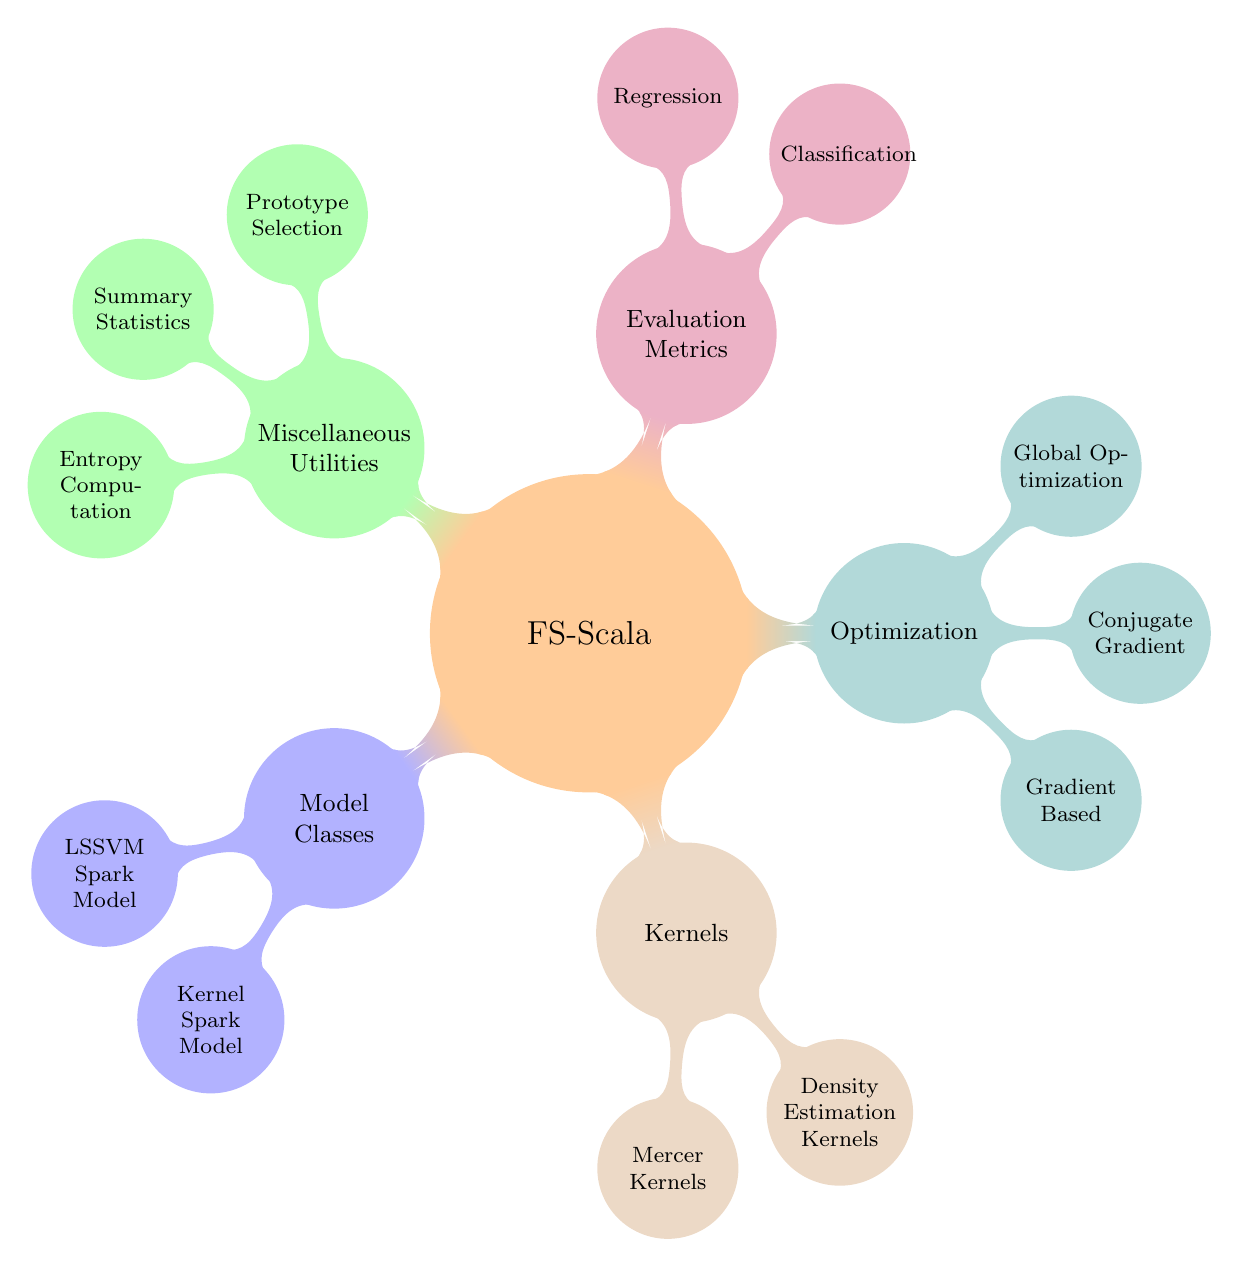
\begin{tikzpicture} [mindmap, grow cyclic, every node/.style=concept, concept color=orange!40, 
    level 1/.append style={level distance=4cm,sibling angle=72},
    level 2/.append style={level distance=3cm,sibling angle=45},]
\node{FS-Scala}
   child [concept color=blue!30]{ node {Model Classes}
        child { node {LSSVM Spark Model}}
        child { node {Kernel Spark Model}}
    }
    child [concept color=brown!30]{ node {Kernels}
        child { node {Mercer Kernels}}
        child { node {Density Estimation Kernels}}
    }
    child [concept color=teal!30]{ node {Optimization}
        child { node {Gradient Based}}
        child { node {Conjugate Gradient}}
        child { node {Global Optimization}}
    }
    child [concept color=purple!30]{ node {Evaluation Metrics}
        child { node {Classification}}
        child { node {Regression}}
    }
    child [concept color=green!30]{ node {Miscellaneous Utilities}
        child { node {Prototype Selection}}
        child { node {Summary Statistics}}
        child { node {Entropy Computation}}
    };

\end{tikzpicture}
\end{adjustbox}
\caption{Schematic structure of FS-Scala}
\label{fig:struct}
\end{figure}



\section{Conclusion}
The final section of the chapter gives an overview of the important results
of this chapter. This implies that the introductory chapter and the
concluding chapter don't need a conclusion.

\lipsum[66]

%%% Local Variables: 
%%% mode: latex
%%% TeX-master: "thesis"
%%% End: 

\chapter{Distributed Computation Support}
\label{cha:3}

\section{Map Reduce}

As discussed above, we use \textit{MapReduce} wherever possible in order to distribute the workload using \textit{Apache Spark}. Due to the primal formulation of the FS-LSSVM, the size of matrix $A =  \hat{\Phi}^{\intercal}_e \hat{\Phi}_e + \frac{\mathit{I}_{m+1}}{\gamma}$ , in the linear system in \eqref{eqfssol} is $(m+1) \times (m+1)$, where $m$ is the number of prototypes selected to construct the kernel matrix in kernel based FS-LSSVM. Procedure \ref{cgmr} outlines the procedure to estimate the parameters $\hat{w},\ \hat{b}$ of the FS-LSSVM model discussed in section \ref{sec:fs}, using the \textit{Conjugate Gradient} algorithm. 

Using \textit{MapReduce}, we calculate $A = \hat{\Phi}^{\intercal}_e \hat{\Phi}_e + \frac{\mathit{I}_{m+1}}{\gamma}$ and $\hat{\Phi}^{\intercal}_e Y$. We use these results to carry out iterations of the Conjugate Gradient updates until the maximum number of iterations is reached.

\begin{algorithm}[t]\label{fmmr}
    \DontPrintSemicolon
    \KwData{$X = [x^i],\ x^i\ \epsilon \ \mathbf{R}^n$, 
    $\hat{\phi} : \mathbf{R}^n \longrightarrow \mathbf{R}^m$, 
    $Y = [y^i], y^i \epsilon \mathbf{R}$}
    \KwResult{$\left ( \hat{\Phi}^{\intercal}_e \hat{\Phi}_e \right ),\ \hat{\Phi}^{\intercal}_e Y$}
    \Begin{
        $MapFn(x, y)$:\;
        \ \   $M \longleftarrow \hat{\phi}(x) \hat{\phi}(x)^T$\;
        \ \   $v \longleftarrow \hat{\phi}(x) \ y$\;
        $emit(M,v)$\;
    }
    \Begin{
        $RedFn((M, v), (M', v'))$:\;
        $emit(M + M', v + v')$\;
    }
    \Begin{
        $(F, v) \longleftarrow MapReduce(X, MapFn, RedFn)$\;
        
        return $(F, v)$\;
    }
\caption{Calculate feature matrices from data using MapReduce: $FeatureMat$}
\end{algorithm}


\begin{algorithm}[t]\label{cgmr}
    \DontPrintSemicolon
    \KwData{$X = [x^i],\ x^i\ \epsilon \ \mathbf{R}^n$, 
    $\hat{\phi} : \mathbf{R}^n \longrightarrow \mathbf{R}^m$, 
    $Y = [y^i], y^i \epsilon \mathbf{R}$, $\gamma$, $\epsilon$}
    \KwResult{$\left( \begin{matrix}
\hat{w}\\ 
\hat{b}
\end{matrix}\right ) = 
\left ( \hat{\Phi}^{\intercal}_e \hat{\Phi}_e + \frac{\mathit{I}_{m+1}}{\gamma} \right )^{-1} \hat{\Phi}^{\intercal}_e Y$}
    \Begin{
        $(F, v) \longleftarrow FeatureMat(X, Y, \hat{\phi}, \gamma)$ \;
        $A \longleftarrow F + \frac{1}{\gamma} \mathbf{I}_{m \times m}$\;
        \BlankLine
        \nl\While{not $max iterations$ and $\Delta(\hat{w}, \hat{b}) \geq \epsilon$}{
            $(\hat{w}_{i+1}, \hat{b}_{i+1}) \longleftarrow CGUpdate(\hat{w}_{i}, \hat{b}_{i}, A, v)$\;
            $\Delta(\hat{w}, \hat{b}) \longleftarrow \left \| \hat{w}_{i+1}  - \hat{w}_{i}\right \|^2 + \left \| \hat{b}_{i+1}  - \hat{b}_{i}\right \|^2$
        }
    }
\caption{Conjugate Gradient: $CG$}
\end{algorithm}


\begin{algorithm}[!htbp]\label{efmr}
    \DontPrintSemicolon
    \KwData{$X_f = [x^i],\ x^i\ \in \ \mathbf{R}^n$, 
    $\hat{\phi} : \mathbf{R}^n \longrightarrow \mathbf{R}^m$, 
    $Y_f = [y^i], y^i \in \mathbf{R}$, $\hat{w}$, $\hat{b}$.}
    \KwResult{score for given fold}
    \Begin{
        $predictLabel(\hat{w}, \hat{b})(x, y)$:\;
        $emit(\hat{w}\cdot x + \hat{b},y)$\;
    }
    \Begin{
        $Vector.fill(length)(IndicatorFn)$:\;
        $vec \longleftarrow (0, ..., 0)_{length} \ map (IndicatorFn)$\;
        $return(vec)$\;
    }
    \Begin{
        $MapScore(score, label)$:\;
        \eIf{label = 1.0}{
            $Pos \longleftarrow Pos + 1$\;
            $tpv \longleftarrow Vector.fill(l)(IndicatorFn(sign(score - thresholds(i)) == 1.0))$\;
            $fpv \longleftarrow Vector.fill(l)(IndicatorFn(false))$\;
        }{
            $Neg \longleftarrow Neg + 1$\;
            $tpv \longleftarrow Vector.fill(l)(IndicatorFn(false))$\;
            $fpv \longleftarrow Vector.fill(l)(IndicatorFn(sign(score - thresholds(i)) == 1.0))$\;
        }
        $emit(tpv,fpv)$\;
    }
    \Begin{
        $RedScore((u, v), (u', v'))$:\;
        $emit(u + u', v + v')$\;
    }
    \Begin{
        $thresholds \longleftarrow List(t_1, t_2, \ldots t_l)$\;
        $Pos \longleftarrow 0$\;
        $Neg \longleftarrow 0$\;
        $scoresLabels \longleftarrow (X_f, Y_f)\ map\ predictLabel(\hat{w}, \hat{b})$\;
        $(tp, fp) \longleftarrow scoresLabels \ map(MapScore) \ reduce(RedScore)$\;
        \BlankLine
        $tp \longleftarrow tp / Pos$
        $fp \longleftarrow fp / Neg$
        $roc \longleftarrow thresholds\ zip(tp\ zip\ fp)$\;
        \BlankLine
        
        return $1 - area(roc)$\;
    }
\caption{Evaluate performance for fold: $evaluateFold$}
\end{algorithm}


\begin{algorithm}\label{cvmr}
    \DontPrintSemicolon
    \KwData{$X = [x^i],\ x^i\ \epsilon \ \mathbf{R}^n$, 
    $\hat{\phi} : \mathbf{R}^n \longrightarrow \mathbf{R}^m$, 
    $Y = [y^i], y^i \epsilon \mathbf{R}$, $\gamma$, folds}
    \KwResult{Cross Validation Performance}
    
    \Begin{
        $(A, v) \longleftarrow FeatureMat(X, Y, \hat{\phi}, \gamma)$ \;
        $score \longleftarrow 0$\;
        \BlankLine
        \nl\For{$i \longleftarrow 1 \ to \ folds $}{
            $(X_i, Y_i) \longleftarrow$ fold i\;
            $(A_i, v_i) \longleftarrow FeatureMat(X_i, Y_i, \hat{\phi}, \gamma)$ \;
            $(\hat{w}, \hat{b}) \longleftarrow CG(A - A_i + \frac{1}{\gamma} \mathbf{I}_{m \times m}, v - v_i)$\;
            $score \longleftarrow score + evaluateFold(\hat{w}, \hat{b}, X_i, Y_i)$\;
        }
        return $score/folds$\;
    }
\caption{Distributed v-Fold Cross-Validation}
\end{algorithm}

% ... and so on until
\npdecimalsign{.}
\nprounddigits{3}
\chapter{Experiments}
\label{cha:n}
The following hardware mentioned in table \ref{table:hardware} is employed to execute \textit{FS-Scala} on a set of benchmark data sets. Machine number 1 is at the Department of Electrical Engineering, KU Leuven. The distributed FS-LSSVM implementation in \emph{FS-Scala} inside a local \emph{Apache Spark} application running concurrently on each core of the host machine.

\begin{table*}[!htbp]
\caption{Hardware Specifications}
\label{table:hardware}
\adjustbox{max width=\textwidth}{
\begin{tabular}{c c c c}
 \textbf{Machine No.} & \textbf{Machine} & \textbf{Configuration} & \textbf{Data Sets} \\
 \hline
 1 & sista-nc-3 & 40 core 64GB RAM & \textit{Adult} and \textit{Forest Cover Type}\\
 2 & Laptop PC & 4 core 8GB RAM & \textit{Magic Gamma}
\end{tabular}
}
\end{table*}

\section{Data Sets}

Experiments are carried out on the \textit{Magic Gamma} Telescope, \textit{Adult} and \textit{Forest Cover Type} data sets available from the UCI Machine Learning Repository \cite{Lichman:2013}. Below we give a short description of each.

\begin{itemize}
\item Magic Gamma: The data is generated by the registration of high speed gamma particles measured by a ground based atmospheric Cherenkov gamma telescope. Each entry consists of 10 numerical attributes and a binary class attribute. 

\begin{table*}[!htbp]
\caption{Magic Gamma Metadata}
\label{table:magicgamma}
\centering
\adjustbox{max width=\textwidth}{
\begin{tabular}{ l l}
%\hline
\textbf{Name} & \textbf{Value}\\
\hline
Training samples & 18792 \\
Test Samples & 228 \\
Features & 10\\
%\hline
\end{tabular}
}
\end{table*}


\item Adult: This is based on a a census study carried out in 1994, the data consists of 6 numerical attributes and 8 categorical attributes. The target attribute is binary class value, which indicates if the given individual has an annual income more than $50 000$\$.

\begin{table*}[!htbp]
\caption{Adult Metadata}
\label{table:adult}
\centering
\adjustbox{max width=\textwidth}{
\begin{tabular}{ l l}
%\hline
\textbf{Name} & \textbf{Value}\\
\hline
Training samples & 29310 \\
Test Samples & 3251 \\
Features & 13\\
%\hline
\end{tabular}
}
\end{table*}


\item Forest Cover Type: This consists of cartographic data collected by the US Forest Service (USFS) on $30 \times 30$ metre cells which have can have seven different forest cover types. For the purposes of the experiments below, a binary classification problem is constructed which consists of recognizing cover type class two from the other cover types. 

\begin{table*}[!htbp]
\caption{Cover Type Metadata}
\label{table:forestcover}
\centering
\adjustbox{max width=\textwidth}{
\begin{tabular}{ l l}
%\hline
\textbf{Name} & \textbf{Value}\\
\hline
Training samples & 523076 \\
Test Samples & 57936 \\
Features & 53\\
%\hline
\end{tabular}
}
\end{table*}

\end{itemize}

\section{Methodology}
The performance of various kernel based FS-LSSVM models is carried out for various values of the experimental parameters listed in table \ref{table:param}. Performance metrics given in table \ref{table:metrics} are computed for each cross validation and used to choose the best performing model during model tuning. To calculate the final performance estimate of each model given the number of prototypes, kernel and grid parameters, each experiment is repeated four times, the mean and standard deviation (in brackets), of the classification accuracy, area under ROC curve and execution time are recorded and presented in tables \ref{table1}, \ref{table2} and \ref{table3} for the \textit{Magic Gamma}, \textit{Adult} and \textit{Forest Cover Type} data sets respectively.

\begin{table*}[!htbp]
\caption{Experiment Parameters}
\label{table:param}
\adjustbox{max width=\textwidth}{
\begin{tabular}{ c l r}
%\hline
\textbf{Name} & \textbf{Meaning} & \textbf{Values} \\
\hline
Kernel & Kernel Type & Linear, RBF, Polynomial, Laplacian \\ 
Prototypes & No. of prototypes & 50, 100, 200\\ 
Global Opt. & Global optimization & gs: Grid Search, csa: Coupled Simulated Annealing\\
Grid Size & Number of grid points  & 2,3,4\\
$nTrials$ & Number of times each experiment is carried out & 4\\
$CGIterations$ & Number of local CG iterations & 35\\
$nFolds$ & Number of folds: fast CV \ref{cvmr}\\
$CSAIterations$ & Number of CSA iterations when used as Global Opt. & 5\\
%\hline
\end{tabular}
}
\end{table*}

\clearpage

\begin{table*}[!htbp]
\caption{Metrics}
\label{table:metrics}
\centering
\adjustbox{max width=\textwidth}{
\begin{tabular}{ c l}
%\hline
\textbf{Name} & \textbf{Meaning}\\
\hline
Accuracy & Classification accuracy on test set averaged over \\
ROC area & avg. area under the ROC curve \\
Execution Time & avg. execution time of FS-LSSVM model tuning in seconds\\
%\hline
\end{tabular}
}
\end{table*}

\section{Results}

\subsection*{Magic Gamma}
The performance of binary FS-LSSVM classifiers on the \textit{MAGIC Gamma} Telescope Data Set obtained from the UCI Machine Learning Repository, are summarized in Table \ref{table1}. FS-LSSVM models trained with polynomial kernels give better classification performance than the RBF and Linear counterparts, on the \textit{MAGIC Gamma} data. Judging from the difference in the performance results between polynomial and linear LSSVM models, it can be said that the \textit{Magic Gamma} data set has weak non linear behavior.
 
\DTLloaddb{magicgamma}{resultsMagicGammaProc.csv}
\begin{table*}[!htbp]
\sisetup{round-mode=places}
\caption{Magic Gamma Test Results}
\begin{center}
\adjustbox{max width=\textwidth}{
\begin{tabular}{l l l l l l l}\label{table1}
\bfseries Kernel & \bfseries Prototypes & \bfseries Global Optimization & \bfseries Grid Size 
& \bfseries Accuracy & \bfseries ROC area & \bfseries Execution Time%
\DTLforeach{magicgamma}{\kernel=kernel,\prototypes=prototypes,
\globaloptimization=globaloptimization,\gridsize=gridsize,
\acc=accuracy,\stdA=stdA,\maxF=maxF1score,
\stdF=stdF,\areaunderROC=areaunderROC,\stdR=stdR,\time=time,\stdT=stdT}%
{%
  \\\kernel & \prototypes & \globaloptimization & \gridsize & 
  $\acc(\stdA)$ & $\areaunderROC(\stdR)$ & $\time(\stdT)$
}%
\end{tabular}
}
\end{center}
\end{table*}

\subsection*{Adult}
The performance of binary FS-LSSVM classifiers on the \textit{Adult} Data Set, are summarized in Table \ref{table2}. FS-LSSVM models trained with exponential kernels give better classification performance than the RBF and Linear counterparts, on the \textit{Adult} data. For both the data sets one sees a pattern emerging that tuning kernel models with CSA gives better results than naive \textit{Grid Search} based hyper-parameter optimization.

\DTLloaddb{adultres}{adultres.csv}
\begin{table*}[!htbp]
\caption{Adult Data Set Test Results}
\begin{center}
\adjustbox{max width=\textwidth}{
\begin{tabular}{l l l l l l l}\label{table2}
\bfseries Kernel & \bfseries Prototypes & \bfseries Global Optimization & \bfseries Grid Size
& \bfseries Accuracy & \bfseries ROC area & \bfseries Execution Time%
\DTLforeach{adultres}{\kernel=kernel,\prototypes=prototypes,
\globaloptimization=globaloptimization,\gridsize=gridsize,
\gridresolution=gridresolution,\acc=accuracy,\stdA=stdA,\maxF=maxF1score,
\stdF=stdF,\areaunderROC=areaunderROC,\stdR=stdR,\time=time,\stdT=stdT}%
{%
  \\\kernel & \prototypes & \globaloptimization & \gridsize & 
  $\acc(\stdA)$ & $\areaunderROC(\stdR)$ & $\time(\stdT)$
}%
\end{tabular}
}
\end{center}
\end{table*}


\subsection*{Forest Cover}
Due to the computational overhead, only CSA based model tuning is employed in the experiments on the \textit{Forest Cover Type} data, yet some clear trends can be observed in table \ref{table3}. It is observed that the Laplacian kernel based models outperform the RBF as well as the linear LSSVMs. This is because the Laplacian kernel relying on the $L_1$ norm is more robust to outliers and leads to a matrix ($A$) with a better condition number, leading CG iterations that converge in fewer iterations.
 
\DTLloaddb{forestcoverproc}{forestcoverproc.csv}
\begin{table*}[!htbp]
\caption{Forest Cover Type Data Set Test Results}
\begin{center}
\adjustbox{max width=\textwidth}{
\begin{tabular}{l l l l l l l}\label{table3}
\bfseries Kernel & \bfseries Prototypes & \bfseries Global Optimization & \bfseries Grid Size 
& \bfseries Accuracy & \bfseries ROC area & \bfseries Execution Time%
\DTLforeach{forestcoverproc}{\kernel=kernel,\prototypes=prototypes,
\globaloptimization=globaloptimization,\gridsize=gridsize,
\gridresolution=gridresolution,\acc=accuracy,\stdA=stdA,\maxF=maxF1score,
\stdF=stdF,\areaunderROC=areaunderROC,\stdR=stdR,\time=time,\stdT=stdT}%
{%
  \\\kernel & \prototypes & \globaloptimization & \gridsize & 
  $\acc(\stdA)$ & $\areaunderROC(\stdR)$ & $\time(\stdT)$
}%
\end{tabular}
}
\end{center}
\end{table*}

%%% Local Variables: 
%%% mode: latex
%%% TeX-master: "thesis"
%%% End: 

\chapter{Conclusions and Future Work}\label{cha:conclusion}

In this thesis, \textit{FS-Scala} a Scala-based implementation of the FS-LSSVM is proposed as a programming framework for working with small and large scale FS-LSSVM models. The current SVM and LSSVM software do not leverage distributed \textit{MapReduce} to implement kernel based SVM/LSSVM models but rather provide support for only linear models in the case of large data sets (\textit{Apache Spark} \cite{Spark:2010}). 

The proposed library \textit{FS-Scala} includes global optimization algorithms like \textit{Grid Search} (GS) and \textit{Coupled Simulated Annealing} (CSA) used to tune FS-LSSVM models. In order to make the tuning of non linear classification models possible on large data sets, a number of performance enhancements are proposed in section \ref{contributions}, which include but not limited to fast v-fold cross validation and feature matrix caching.

In chapter \ref{cha:n}, \textit{FS-Scala} is applied on a number of benchmark data sets (i.e. \textit{Magic Gamma}, \textit{Adult} and \textit{Forest Cover Type}) and the performance and model tuning time are recorded. It is observed that our implementation enables scalable training, tuning and evaluation of LSSVM models, while still providing flexibility to tweak various underlying data processing infrastructure. We conclude by discussing ideas for future research work and further improvements to \textit{FS-Scala}. 

\section*{Future Work}

Further research/improvements on \textit{FS-Scala} can be done in two proposed directions.

\begin{itemize}
\item Experiments of large scale commodity clusters:
Simulations were carried on a \emph{Apache Spark} standalone cluster which runs tasks concurrently over the different cores of the parent machine. But it is also possible to scale this process even further for greater computational benefits by using large commodity clusters as provided by cloud computing providers.

\item Simultaneous evaluation of multiple model instances:
During a particular v-fold cross validation operation only a single model instance (configuration of hyper-parameters) is trained and  evaluated, therefore to evaluate a $k \times k$ grid, $k^2$ v-fold cross validations must be carried out. Substantial improvements can be achieved if we can train and do v-fold CV on multiple model instances using only a single pass through the training data, leading to a new and exciting area of research in large scale FS-LSSVM model tuning. 
\end{itemize}

% If you have appendices:
\appendixpage*          % if wanted
\appendix
\chapter{FS-Scala Class Hierarchies}
\label{app:A}
Figures \ref{fig:modelUML} and \ref{fig:modelUML1} depict the class hierarchy structures of the core and optimization modules respectively, we can discuss their role in depth.

\section{Core Components}
The core module consists of a set of classes which all originate from a base abstraction called \textit{Model}. It also has classes \textit{ParameterizedLearner} and \textit{LinearModel} representing the core behaviors of parameter based Machine Learning models which form a large chunk of current learning techniques. By using generic typing inherent in the Scala language, one is able to separate the logic of a model from the details of the underlying data infrastructure. This is particularly relevant due to the explosion of data processing frameworks and systems like graph databases, Apache Spark, key value stores, column oriented databases, etc.

\subsection*{Kernel Functions and Kernel Based Models}
The kernel module contains implementations of SVM kernels and AFE. The class \textit{KernelizedModel} defines kernel based linear models which use the \textit{GlobalOptimizer} class to tune values of hyper-parameters. The actual implementation of the \textit{Automatic Feature Extraction} is abstracted out in the parent classes, thereby reducing the effort of writing new SVM kernels to merely expressing their evaluation functions.


\begin{figure}[!ht]
\begin{adjustbox}{max width=0.85\textwidth}
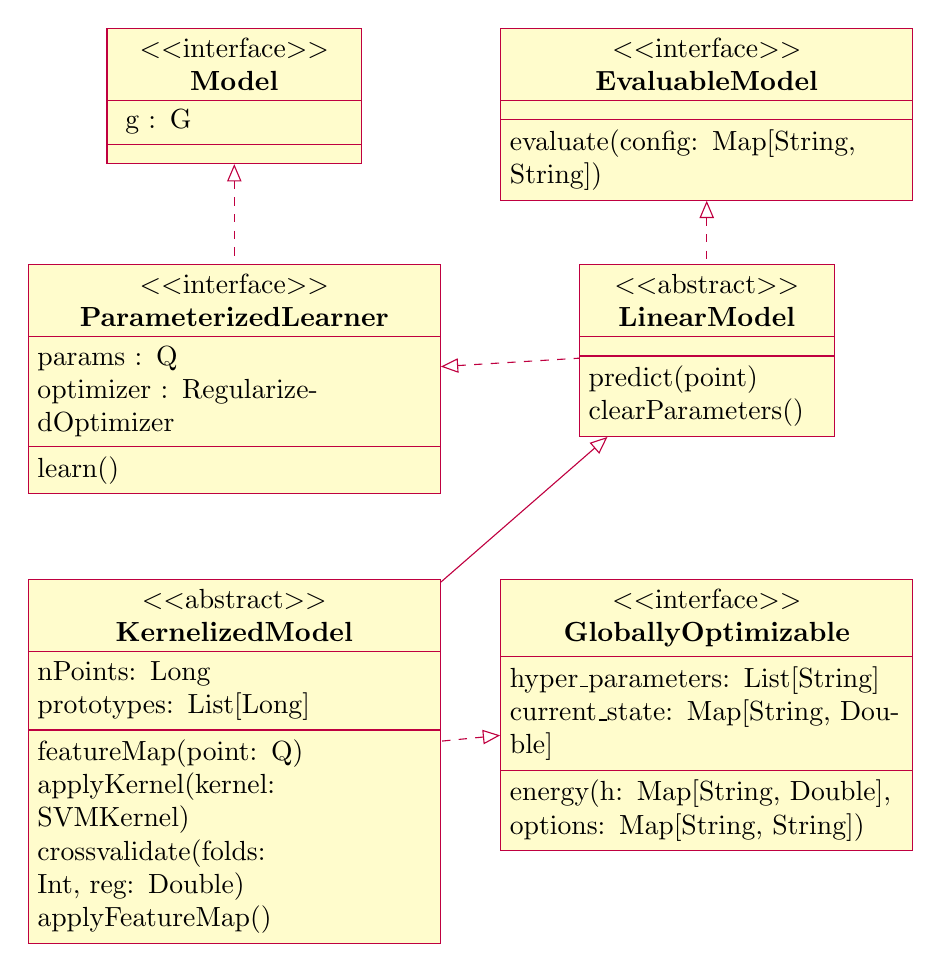
\begin{tikzpicture}
    \begin{interface}[text width =3 cm]{Model}{0 ,0}
        \attribute { g : G }
    \end{interface}
    
    \begin{interface}[]{ParameterizedLearner}{ 0 , -3}
        \implement{Model}
        \attribute{params : Q}
        \attribute{optimizer : RegularizedOptimizer}
        \operation{learn() }
    \end{interface}
    
    \begin{interface}[]{EvaluableModel}{ 6 , 0}
        \operation{evaluate(config: Map[String, String]) }
    \end{interface}
    
    \begin{abstractclass}[text width =3 cm]{LinearModel}{6 , -3}
        \implement{ParameterizedLearner}
        \implement{EvaluableModel}
        \operation{predict(point) }
        \operation{clearParameters() }
    \end{abstractclass}
    
    \begin{interface}[]{GloballyOptimizable}{ 6 , -7}
        \attribute{hyper\_parameters: List[String]}
        \attribute{current\_state: Map[String, Double]}
        \operation{energy(h: Map[String, Double], options: Map[String, String]) }
    \end{interface}
    
    \begin{abstractclass}[]{KernelizedModel}{0 , -7}
        \inherit{LinearModel}
        \implement{GloballyOptimizable}
        \attribute{nPoints: Long}
        \attribute{prototypes: List[Long]}
        \operation{featureMap(point: Q)}
        \operation{applyKernel(kernel: SVMKernel) }
        \operation{crossvalidate(folds: Int, reg: Double)}
        \operation{applyFeatureMap()}
    \end{abstractclass}
    
\end{tikzpicture}
\end{adjustbox}
\caption{Class Hierarchy of Core Models API}
\label{fig:modelUML}
\end{figure}

\section{Optimization Methods}
Parametric models in FS-Scala have an embedded optimization object which is inherits from the \textit{Optimizer} interface. Implementations of Conjugate Gradient and Gradient Descent are provided in the optimization module. New optimization algorithms can be added by inheriting from the top level \textit{Optimizer} interface or the \textit{RegularizedOptimizer} abstract class in case one is working with parametric models which involve regularization. Another important component of the optimization module is the \textit{GlobalOptimizer} interface which acts as a skeleton for implementing gradient free global optimization algorithms.

\begin{figure}[!ht]
\begin{adjustbox}{max width=0.85\textwidth}
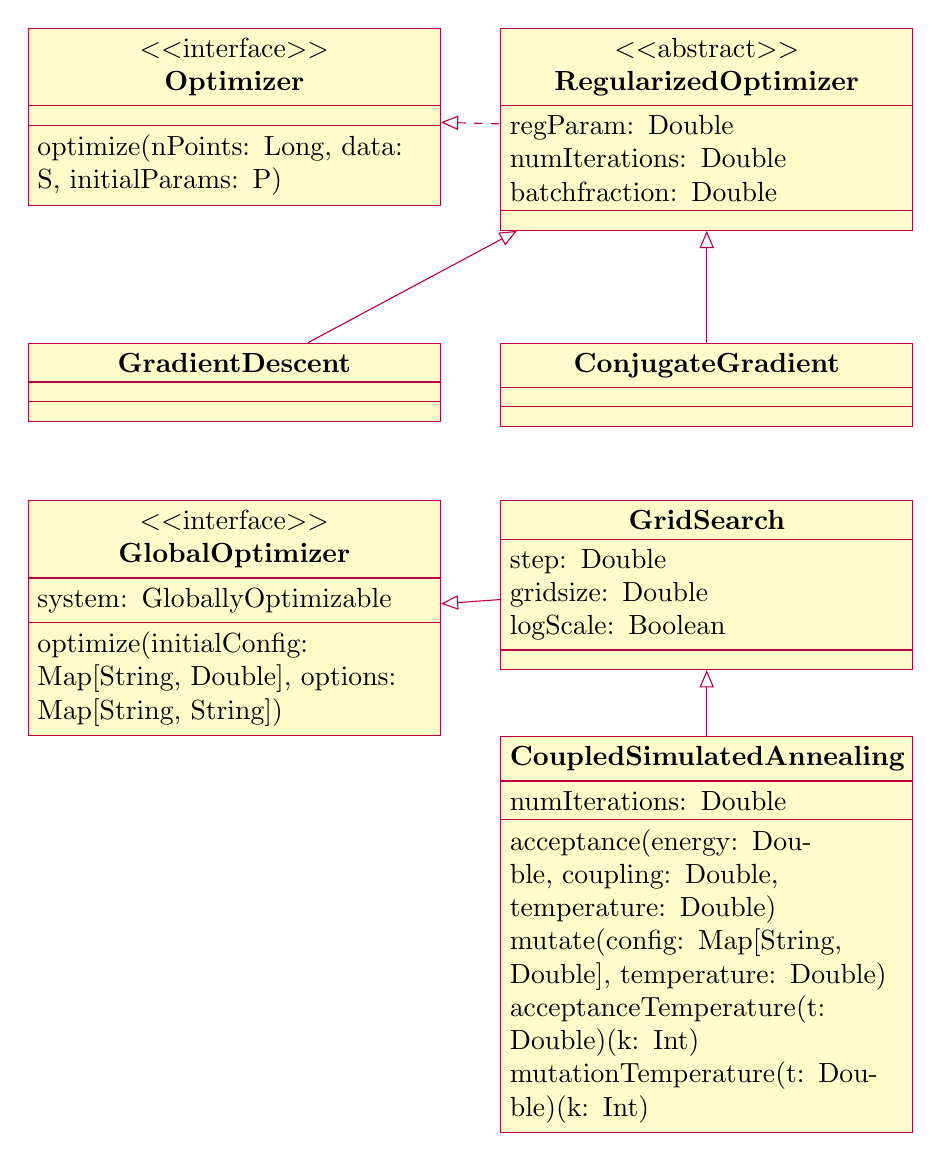
\begin{tikzpicture}
    \begin{interface}[]{Optimizer}{0 ,0}
        \operation{optimize(nPoints: Long, data: S, initialParams: P)}
    \end{interface}
    
    \begin{abstractclass}[]{RegularizedOptimizer}{6 , 0}
        \implement{Optimizer}
        \attribute{regParam: Double}
        \attribute{numIterations: Double}
        \attribute{batchfraction: Double}
    \end{abstractclass}
    
    \begin{class}[]{GradientDescent}{ 0 , -4}
        \inherit{RegularizedOptimizer}
    \end{class}
    
    \begin{class}[]{ConjugateGradient}{6 , -4}
        \inherit{RegularizedOptimizer}
    \end{class}
    
    \begin{interface}[]{GlobalOptimizer}{ 0 , -6}
        \attribute{system: GloballyOptimizable}
        \operation{optimize(initialConfig: Map[String, Double], options: Map[String, String])}
    \end{interface}
    
    \begin{class}[]{GridSearch}{6 , -6}
        \inherit{GlobalOptimizer}
        \attribute{step: Double}
        \attribute{gridsize: Double}
        \attribute{logScale: Boolean}
    \end{class}
    
    \begin{class}[]{CoupledSimulatedAnnealing}{6 , -9}
        \inherit{GridSearch}
        \attribute{numIterations: Double}
        \operation{acceptance(energy: Double, coupling: Double, temperature: Double)}
        \operation{mutate(config: Map[String, Double], temperature: Double)}
        \operation{acceptanceTemperature(t: Double)(k: Int)}
        \operation{mutationTemperature(t: Double)(k: Int)}
    \end{class}
    
    
    
\end{tikzpicture}
\end{adjustbox}
\caption{Class Hierarchy of Optimization API}
\label{fig:modelUML1}
\end{figure}


%%% Local Variables: 
%%% mode: latex
%%% TeX-master: "thesis"
%%% End: 

% ... and so on until
\backmatter
% The bibliography comes after the appendices.
% You can replace the standard "abbrv" bibliography style by another one.
\bibliographystyle{abbrv}
\bibliography{references}

\end{document}

%%% Local Variables: 
%%% mode: latex
%%% TeX-master: t
%%% End: 
